\documentclass[11pt,oneside,letterpaper]{article}

% graphicx package, useful for including eps and pdf graphics
\usepackage{graphicx}
\DeclareGraphicsExtensions{.pdf,.png,.jpg}

% basic packages
\usepackage{color}
\usepackage{parskip}
\usepackage{float}

% text layout
\usepackage{geometry}
\geometry{textwidth=15cm} % 15.25cm for single-space, 16.25cm for double-space
\geometry{textheight=22cm} % 22cm for single-space, 22.5cm for double-space

% helps to keep figures from being orphaned on a page by themselves
\renewcommand{\topfraction}{0.85}
\renewcommand{\textfraction}{0.1}

% bold the 'Figure #' in the caption and separate it with a period
% Captions will be left justified
\usepackage[labelfont=bf,labelsep=period,font=small]{caption}

% review layout with double-spacing
%\usepackage{setspace}
%\doublespacing
%\captionsetup{labelfont=bf,labelsep=period,font=doublespacing}

% cite package, to clean up citations in the main text. Do not remove.
\usepackage{cite}
%\renewcommand\citeleft{(}
%\renewcommand\citeright{)}
%\renewcommand\citeform[1]{\textsl{#1}}

% Remove brackets from numbering in list of References
\renewcommand\refname{\large References}
\makeatletter
\renewcommand{\@biblabel}[1]{\quad#1.}
\makeatother

\usepackage{authblk}
\renewcommand\Authands{ \& }
\renewcommand\Authfont{\normalsize \bf}
\renewcommand\Affilfont{\small \normalfont}
\makeatletter
\renewcommand\AB@affilsepx{, \protect\Affilfont}
\makeatother

% notation
\usepackage{amsmath}
\usepackage{amssymb}

%%% TITLE %%%
\title{\vspace{1.0cm} \Large \bf
ncov-forecasting-fit (title TBD)
}

\author[1,2]{Eslam Abousamra*}
\author[1,3]{Marlin Figgins*}
\author[1,2,4]{Trevor Bedford}

\affil[1]{Vaccine and Infectious Disease Division, Fred Hutchinson Cancer Center, Seattle, WA, USA}
\affil[2]{Department of Epidemiology, University of Washington, Seattle, WA, USA}
\affil[3]{Department of Applied Mathematics, University of Washington, Seattle, WA, USA}
\affil[4]{Howard Hughes Medical Institute, Seattle, WA, USA}


\date{}

\begin{document}

\maketitle

%%% ABSTRACT %%%
\begin{abstract}

Todo

\end{abstract}

%%% INTRODUCTION %%%
\section*{Introduction}

Modeling infectious diseases plays a key role in estimating the emergence of epidemics.
Understanding the trends and characteristics of emerging epidemics can guide public health officials to control their spread [1].
Epidemiologists face a multitude of challenges in order to provide accurate and timely predictions of disease spread.
More recently, with the deluge of data from various sources, issues with data arise regarding quantity, near-real-time accessibility, and quality.
Data integration from different temporal and geographical? leads to issues with reporting bias, submission delays, and back-filling of disease occurence especially with a larger geographical scale [2].
Thus, the quantities and the availability of genomic sequencing data differ depending on the date of observation and forecasting in varying geographical regions being studied.
This variability in sequences availability can have a significant impact on the accuracy and reliability of forecasting efforts using mathematical models.
Furthermore, different modeling approaches may have varying levels of sensitivity to imperfections or limitations in the data.  
Thereby, it is essential to take these factors into account when using mathematical models to make predictions, as they can impact the accuracy and reliability of the model's output [2].



*Challenges

Mathematical models elucidate disease processes and have been sought to assess the risk and framing the response to emerging pathogens. 
Representation of disease mechanisms and spread from genomic sequences can not only help us forecast disease occurrence and pathogen frequencies, but also
uncover the inherent characteristics of emerging pathogens and compare potential mechanisms of spread and persistence in the population [3].
The validity and reliability of these mathematical models are dependent on the quality and quantity of data used for the model.
With the emergence of novel pathogens, real-time data scarcity represent a real challenge to accurate forecasts as it leads to 
increased uncertainty in identifying and forecasting epidemic trends [3].



The need for accurate predictions of epidemic trajectories led to development of "nowcasting" approaches, i.e forecasting on a short-term scale which handles data pitfalls differently. 



* Common Methods to forecast from sequences





* How different models handle imperfect data








I use Google Scholar format for citation style with first author, year and first word of title, ala \cite{hadfield2018nextstrain}.

%%% METHODS %%%
\section*{Methods}

Todo

%%% RESULTS %%%
\section*{Results}

I put figures into a `/figures' directory and use semantic labeling ala (Figure~\ref{example_predictions}).

%%% map %%%
\begin{figure}[h]
	\centering
	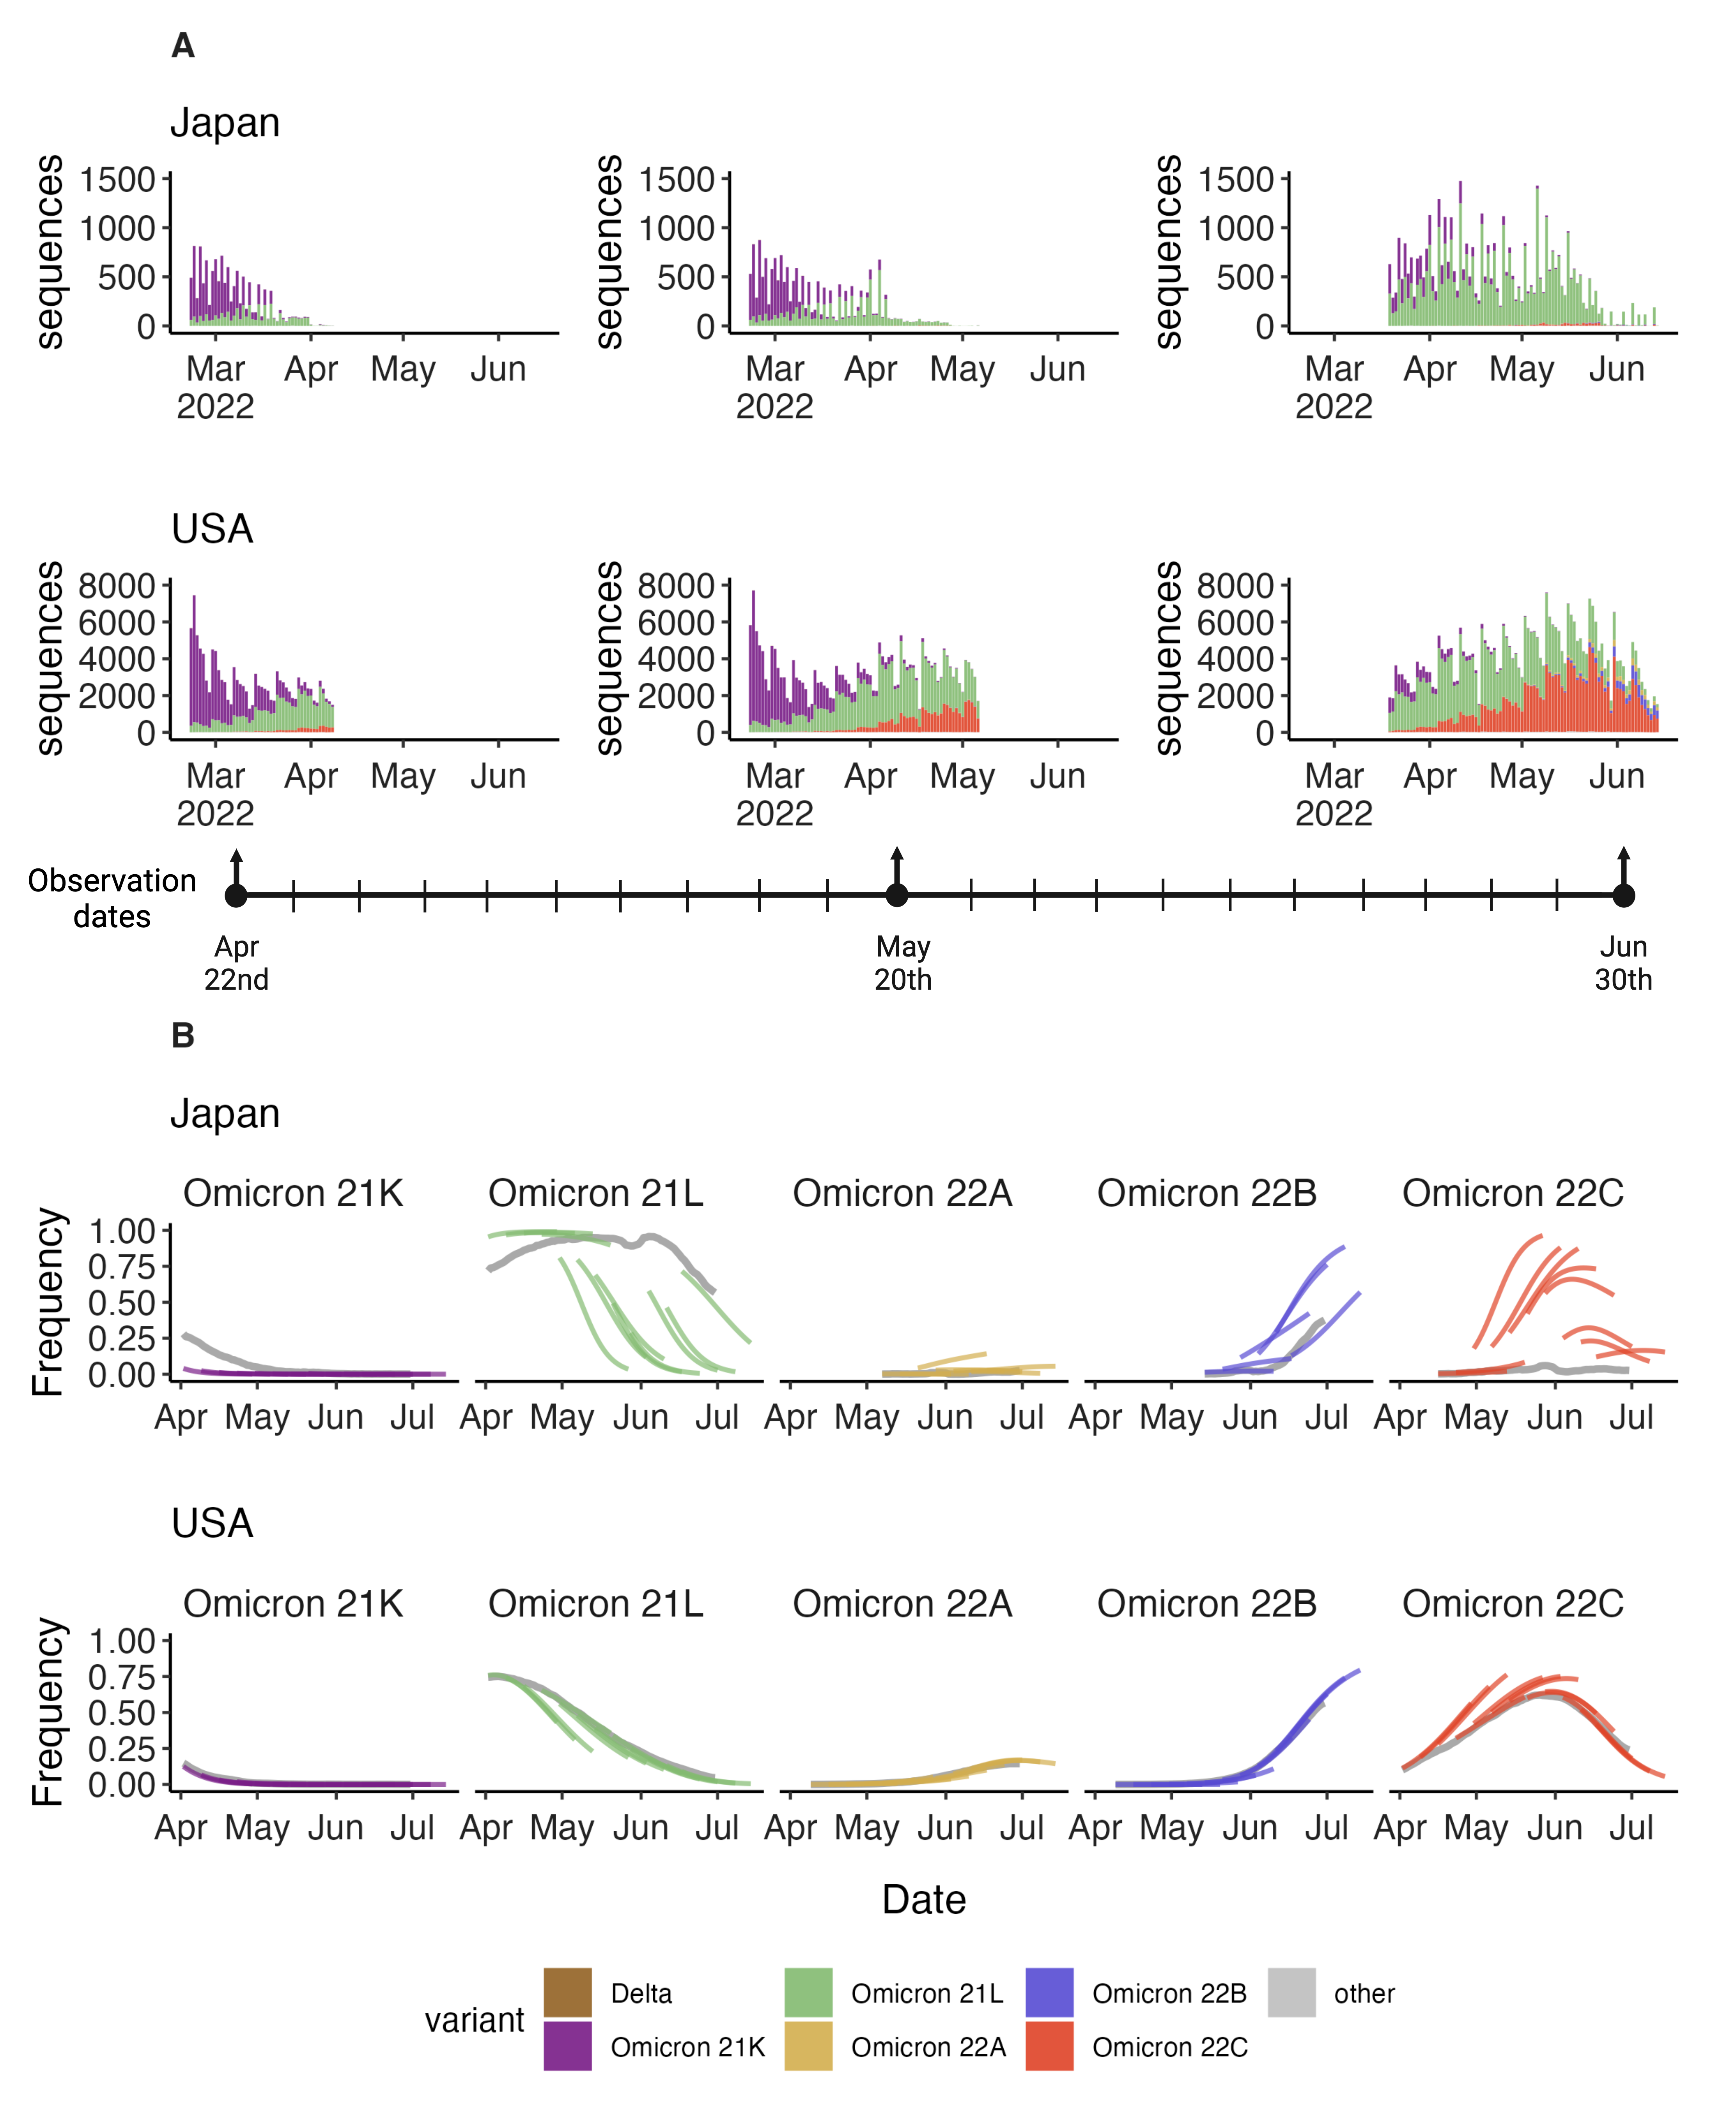
\includegraphics[width=1.0\textwidth]{figures/example_predictions}
	\caption{\textbf{Example data and predictions for Japan and the USA.}
	Further legend here.
	}
	\label{example_predictions}
\end{figure}


\begin{figure}[h]
	\centering
	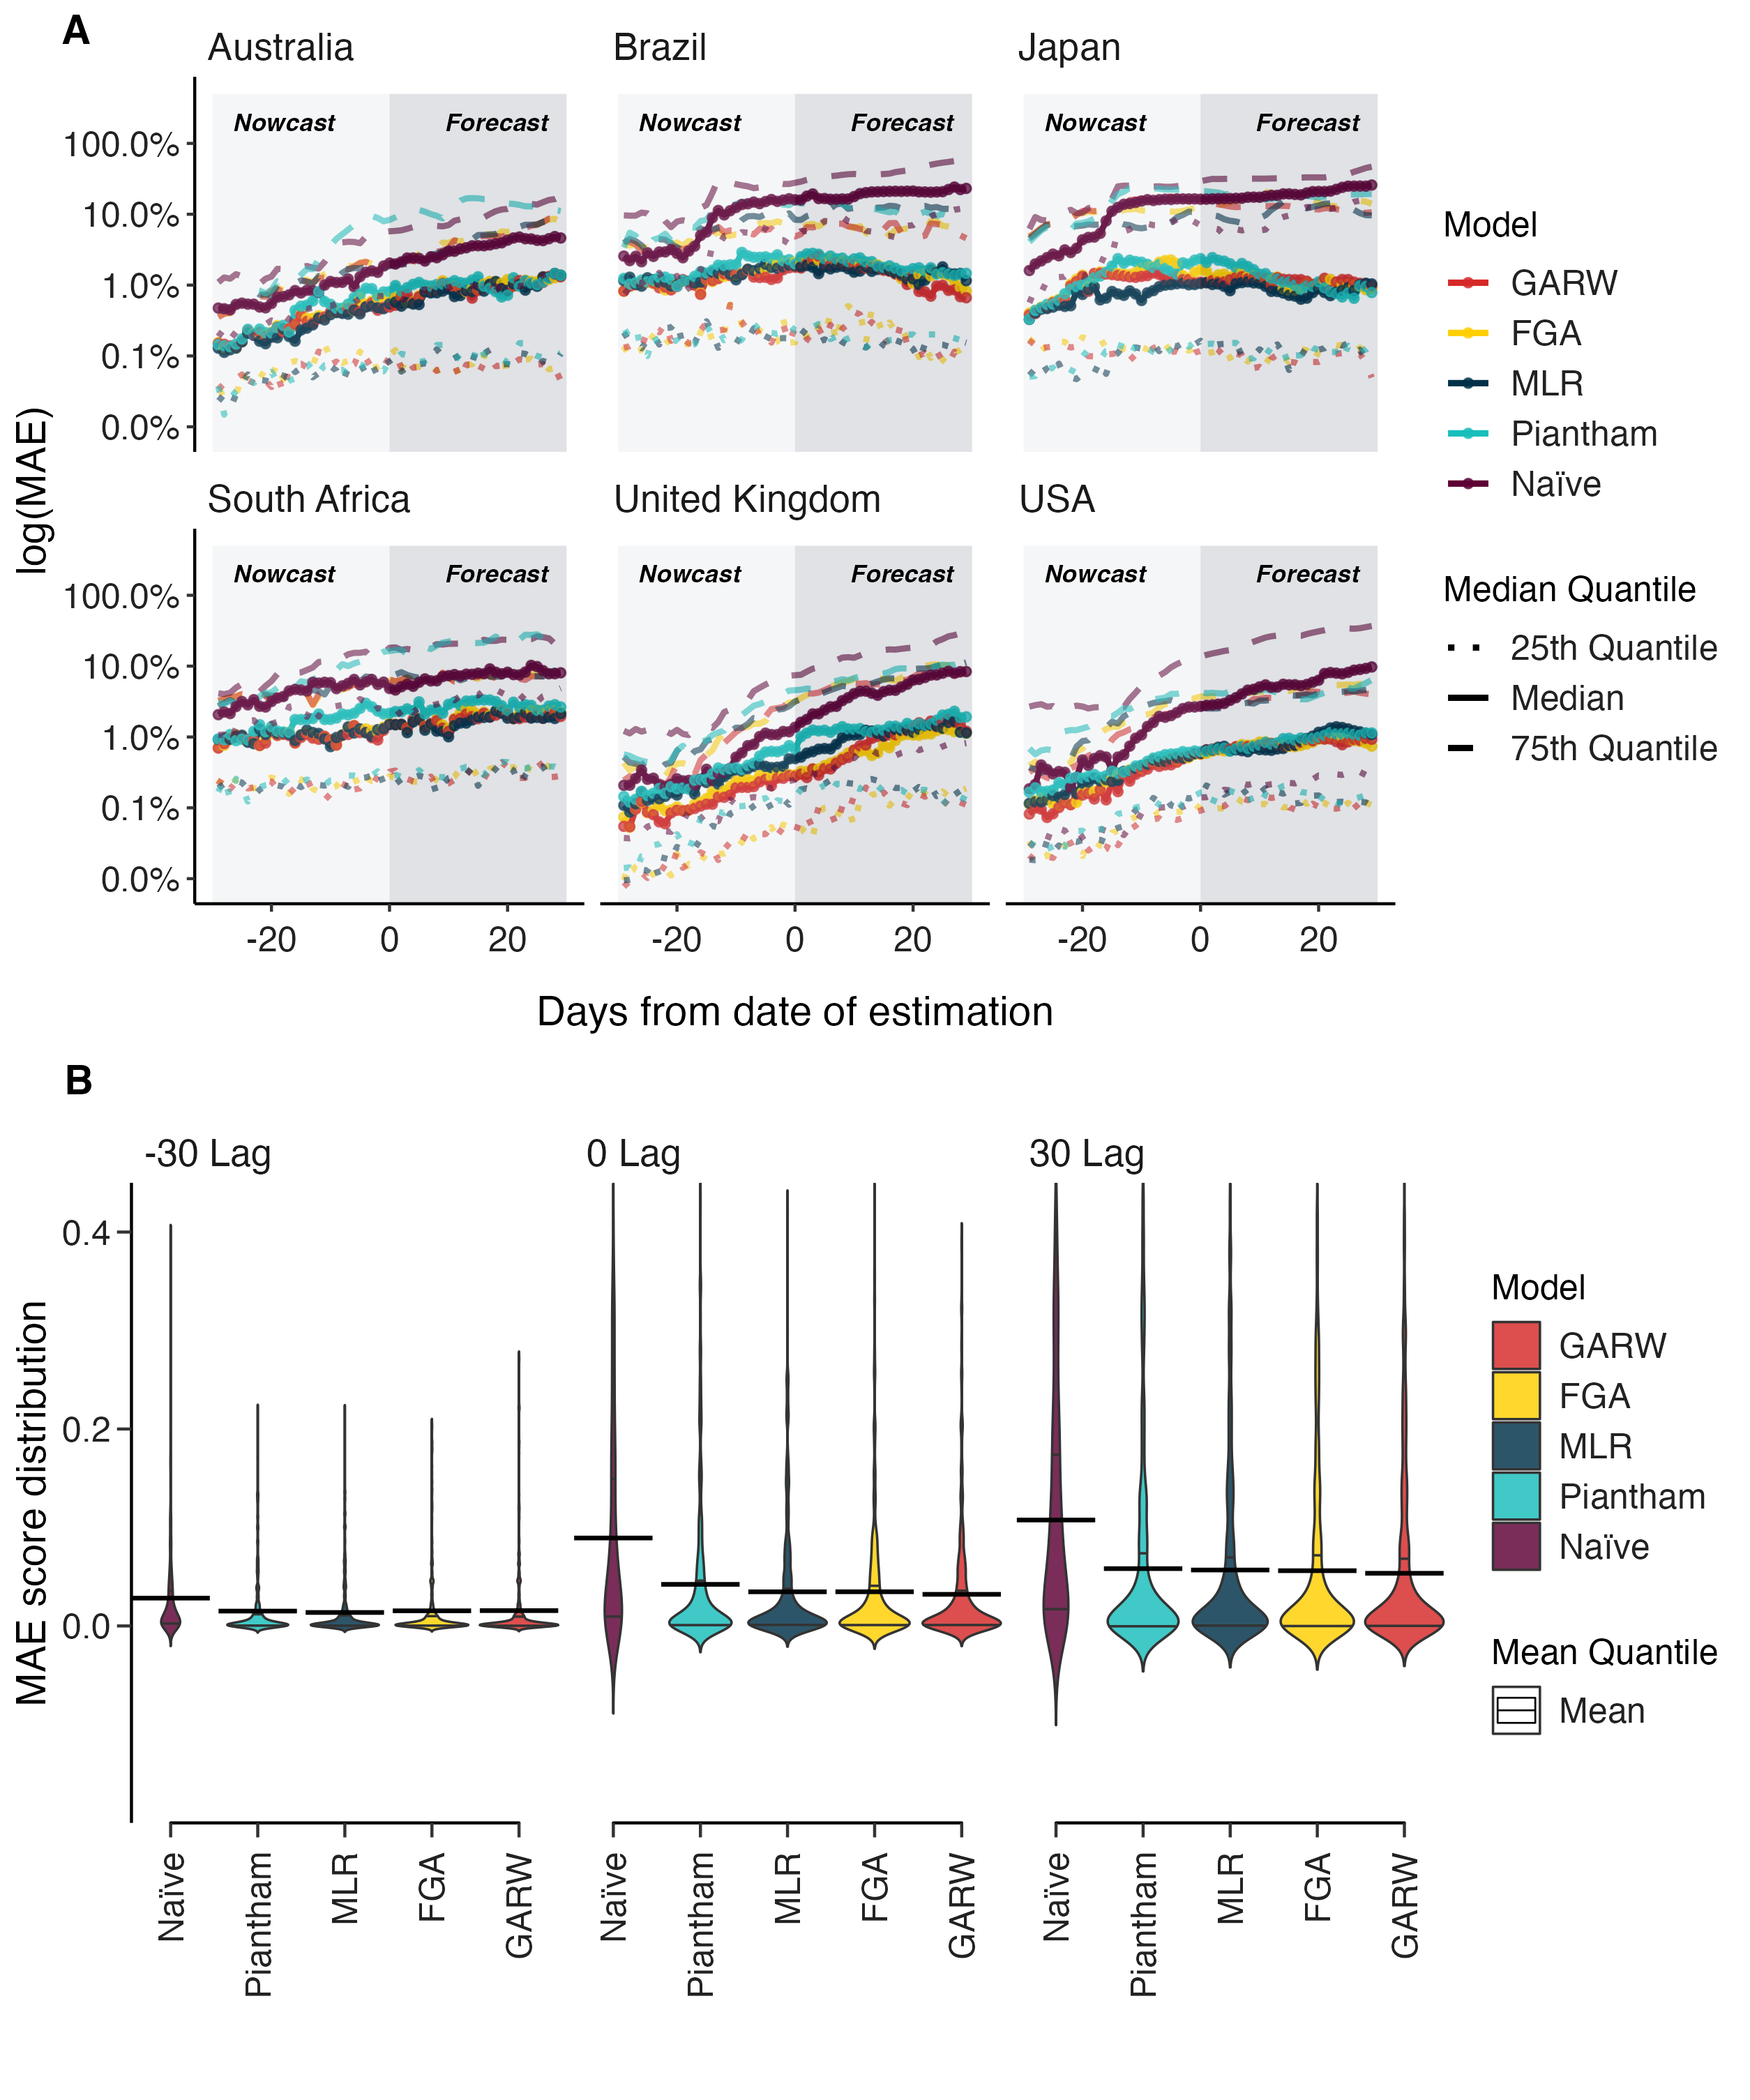
\includegraphics[width=1.0\textwidth]{figures/Figure2.png}
	\caption{\textbf{MAE estimates based on date of estimation.}
	Further legend here.
	}
	\label{Figure 2}
\end{figure}


\begin{figure}[h]
	\centering
	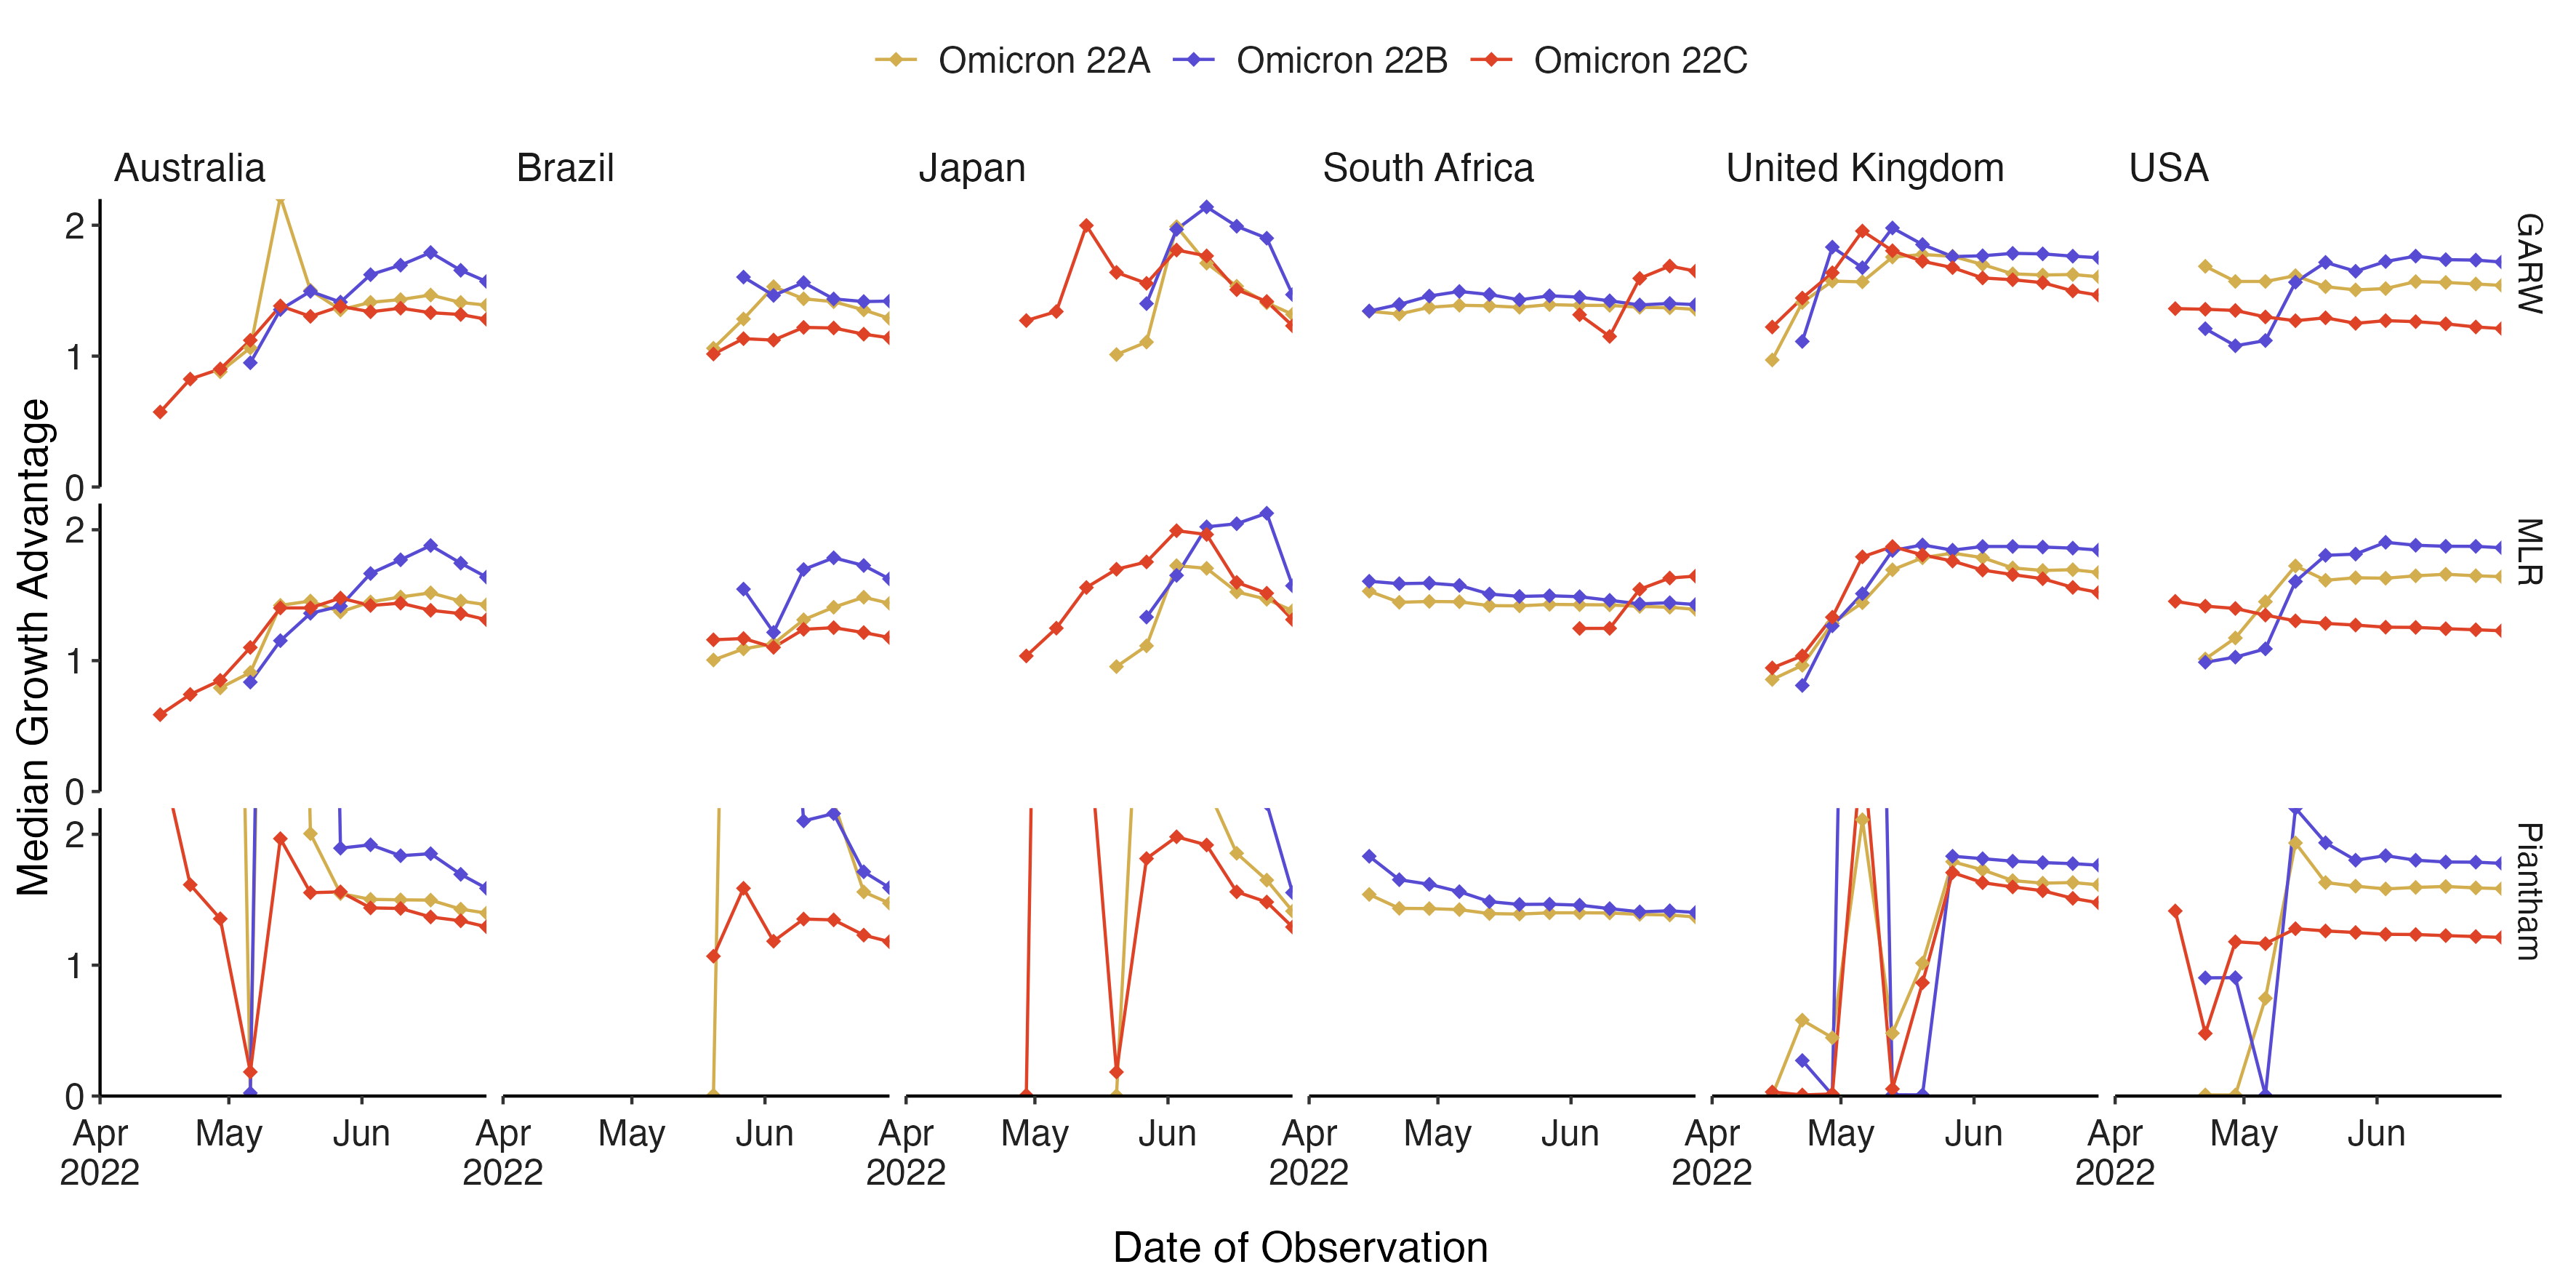
\includegraphics[width=1.0\textwidth]{figures/Figure3.png}
	\caption{\textbf{Growth Advantage of variants over time}
	Further legend here.
	}
	\label{Figure 2}
\end{figure}







%%% DISCUSSION %%%
\section*{Discussion}

Todo

%%% REFERENCES %%%
\bibliographystyle{plos}
\bibliography{ncov-forecasting-fit}

\end{document}
